\RequirePackage[2020-02-02]{latexrelease}

%\documentclass[9pt,twocolumn,twoside]{cidlab-draft}\templatetype{cidlab-invited}\author[a,b,c]{Alexander Etz}
\author[b,c]{Adriana F.\ Ch\'avez De la Pe\~na}
\author[b,c]{Luis Baroja}
\author[b,c]{Kathleen Medriano}
\author[b,c,d,*]{Joachim Vandekerckhove}

\affil[a]{Department of Psychology, University of Texas, Austin}
\affil[b]{Department of Cognitive Sciences, University of California, Irvine}
\affil[c]{Department of Statistics, University of California, Irvine}
\affil[d]{Department of Logic and Philosophy of Science, University of California, Irvine}

\leadauthor{Etz} 

\authorcontributions{All authors contributed to the final draft. Author ORCiD:
AE=0000-0000-0000-0000, AFCP=0000-0000-0000-0000, KM=0000-0000-0000-0000, JLB=0000-0000-0000-0000, JV=0000-0003-2600-5937}
\authordeclaration{This work was supported by National Science Foundation grants \#1658303, \#1850849, and \#2051186. The authors declare no conflicts of interest.}
\correspondingauthor{\textsuperscript{*}Correspondence concerning this article should be addressed to Joachim Vandekerckhove (joachim@uci.edu).}
\equalauthors{}

% Keywords are not mandatory, but authors are strongly encouraged to provide them. If provided, please include two to five keywords, separated by the pipe symbol, e.g:
\keywords{Highest-density interval $|$ ROPE $|$ Incoherence $|$ Bayesian inference $|$ Bayes factor} 

\dates{Draft of \today{}.  Planned outlet: \textit{Psychological Methods}.}
%\dates{Draft of \today{}.  Planned outlet: \textit{Computational Brain \& Behavior}.}
%\dates{This is the author final version of the article.}


\begin{abstract} 
The Bayesian HDI+ROPE decision rule is an increasingly common approach to testing null parameter values. 
The decision procedure involves a comparison between a posterior highest density interval (HDI) and a pre-specified region of practical equivalence (ROPE). One then accepts or rejects the null parameter value depending on the overlap (or lack thereof) between these intervals. 
Here we demonstrate, both theoretically and through examples, that this procedure is logically incoherent.
Because the HDI is not transformation invariant, the ultimate inferential decision depends on statistically arbitrary and scientifically irrelevant properties of the statistical model.
The incoherence arises from a common confusion between probability density and probability proper.  The HDI+ROPE procedure relies on characterizing posterior densities as opposed to being based directly on probability. 
We conclude with recommendations for alternative Bayesian testing procedures that do not exhibit this pathology and provide a ``quick fix'' in the form of quantile intervals.
\end{abstract}
\documentclass[man]{apa}\abstract{The Bayesian HDI+ROPE decision rule is an increasingly common approach to testing null parameter values. 
The decision procedure involves a comparison between a posterior highest density interval (HDI) and a pre-specified region of practical equivalence (ROPE). One then accepts or rejects the null parameter value depending on the overlap (or lack thereof) between these intervals. 
Here we demonstrate, both theoretically and through examples, that this procedure is logically incoherent.
Because the HDI is not transformation invariant, the ultimate inferential decision depends on statistically arbitrary and scientifically irrelevant properties of the statistical model.
The incoherence arises from a common confusion between probability density and probability proper.  The HDI+ROPE procedure relies on characterizing posterior densities as opposed to being based directly on probability. 
We conclude with recommendations for alternative Bayesian testing procedures that do not exhibit this pathology and provide a ``quick fix'' in the form of quantile intervals.}

\shorttitle{Transformation incoherence}

\author{Alexander Etz$^{abc}$,
Adriana F.\ Ch\'avez De la Pe\~na$^{bc}$,
Luis Baroja$^{bc}$,
Kathleen Medriano$^{bc}$,
and
Joachim Vandekerckhove$^{bc}$}

\affiliation{%
$^{a}$ Department of Psychology UT Austin\\
$^{b}$ Department of Cognitive Sciences, UC Irvine\\
$^{c}$ Department of Statistics, UC Irvine}

\leftheader{Etz}

\newcommand{\hdr}{HDRP}

\title{On the transformation incoherence of the HDI+ROPE testing procedure}

\usepackage{
    amsmath,amssymb,amsfonts,
    centernot,csquotes,
    epsfig,epstopdf,epigraph,
    graphicx,
    listings,
    longtable,
    mathtools,
    subfig,
    todonotes,
    tikz,
    url}
\usepackage[super]{nth}
\usepackage[english]{babel}

\newcommand{\jv}[1]{\todo[inline,color=lime]{#1 -\textit{jv}}}
\newcommand{\afcp}[1]{\todo[inline,color=orange]{Adri: #1 }}


\lstdefinestyle{rstyle}{
   language=R,
   basicstyle=\ttfamily\small,
   commentstyle=\color{green!50!black},
   keywordstyle=\color{blue},
   stringstyle=\color{red},
   numbers=left,
   numberstyle=\tiny\color{gray},
   stepnumber=1,
   frame=single,
   breaklines=true,
   showstringspaces=false
}

\newcommand\blfootnote[1]{%
  \begingroup
  \renewcommand\thefootnote{}\footnote{#1}%
  \addtocounter{footnote}{-1}%
%  \endgroup
}



\newcommand{\citealp}[1]{\citeNP{#1}}
\newcommand{\citet}[1]{\citeA{#1}}
\newcommand{\citeyearpar}[1]{\citeyear{#1}}

\makeatletter
\def\citep{%
   \@ifnextchar[%
     {\citep@i}
     {\citep@i[]}%
}
\def\citep@i[#1]{%
   \@ifnextchar[%
     {\citep@ii{#1}}
     {\citep@ii{#1}[]}%
}
\def\citep@ii#1[#2]#3{%
  \cite<#1>[#2]{#3}%
}
\makeatother

\newcommand{\M}{\mathcal{M}}
\DeclareMathOperator*{\argmin}{arg\,min}
\DeclareMathOperator*{\argmax}{arg\,max}
\newcommand{\oddss}{\text{odds}}
\newcommand{\logit}{\text{logit}}

\newcommand{\ora}[1]{{#1}}
\newcommand{\blu}[1]{{#1}}

\def\driftangle{\theta}
\def\nondecisiontime{\tau}
\def\driftlength{\delta}
\def\boundary{\eta}
\def\mux{\mu_x}
\def\muy{\mu_y}
\def\polar{\text{CDDM}_\circ}
\def\cartn{\text{CDDM}_+}

\graphicspath{{./p/}}

\begin{document}

\maketitle

\noindent The crisis of confidence in psychological science has reinflamed historical controversies surrounding the enterprise of statistical hypothesis testing.  Classical null hypothesis significance testing (NHST) has been the target of the majority of these criticisms, including that it is overly dichotomous \cite{gibson2021}, easily ``hackable'' \cite{SimmonsEtAl2011}, it can only reject and not accept the null hypothesis \cite{Rouder2009ttest}, that null hypotheses are false \textit{a priori} \cite{Cohen1994,mcshane2019}, and that it answers the wrong question because estimation is more useful \cite{Cumming2014}. 
\jv{This is a note.}

Alternative methods have been proposed. One prominent example is the so-called HDI+ROPE procedure (henceforth, \hdr{}) introduced by \citeA{Kruschke2011,Kruschke2013} as a superseding alternative to classical NHST.  

While we are strong proponents of the Bayesian statistical paradigm \cite{EtzSI,Vandekerckhove2018} in which \hdr{} is based, we will argue here that \hdr{} is flawed and should be avoided, on grounds similar to the above objections to NHST.  Specifically, \hdr{} can lead to inconsistent inferences that depend critically on highly arbitrary choices that must be made by the analyst about how to represent the model. 

In what follows we will first informally describe the \hdr{} with a fictional scenario that highlights its problematic nature. The example will demonstrate that multiple researchers using the \hdr{} can come to different conclusions despite employing mathematically equivalent models, priors, and data. 

To give insight into why the inconsistent inferences using the \hdr{} occur, we will discuss the formal decision-theoretical properties of the method. The crucial flaw we highlight is that different, but otherwise mathematically equivalent, representations of a hypothesis test do not lead to equivalent inferences. We show that this pathology is due to the \hdr{}'s reliance on probability density to determine which parameter values are ``most plausible.'' However, unlike probability (which requires that equivalent sets must have equal probabilities), probability density values depend on how we label the parameters of a model.  Differently put, \textit{sets of parameter values with high density in one representation of the model may have low density in another}. As a result, \hdr{} can simultaneously conclude that the null hypothesis \textit{is} and \textit{is not} to be rejected, which is logically incoherent.

Finally, we propose an easy-to-implement modification of the \hdr{} that resolves the current pathology and achieves coherence. The solution is to use a test that is based on probability rather than probability density. 


\section*{Introduction to the \hdr{}}

\afcp{The rope is mentioned in the first paragraph before it is introduced (second paragraph)}
The \hdr{} is similar in procedure to the broader category of equivalence tests \cite{RogersEtAl1993}, which can be characterized as extensions of point-null tests into tests of equivalence regions.
However, the \hdr{} only uses the rope as a means to test a point null and does not entail acceptance or rejection of the entire region. The \hdr{} is therefore more similar in logic to other point null tests.

The \hdr{} is conducted as follows \cite{Kruschke2011}.  
First, determine a parameterized model for the data and specify prior distributions for all parameters. 
Then, specify the null hypothesis of interest as one particular parameter value: some specific value of the parameter that is considered especially important, such as a correlation being zero.
Then, specify a ``region of practical equivalence'' (ROPE) around the null value, containing those parameter values that are considered only negligibly different from it for practical purposes.
Then, collect data and obtain the posterior distribution of the parameter of interest. For this step, it is necessary to choose a parameterization of the model to be used for the test. 
From this posterior, then construct a $(100\alpha)\%$ highest-density interval (HDI), which is an interval in which every value has higher posterior density than any outside the interval and which contains $(100\alpha)\%$ of the posterior mass.

Then, finally, if the HDI and ROPE do not overlap, reject the null hypothesis for practical purposes. If the ROPE encompasses the entire HDI, accept the null for practical purposes. If the ROPE and HDI partially overlap, reserve judgment about the status of the null hypothesis. 


\subsection*{A fictional example}
    
Avery, Blair, and Cassidy are triplets who are training their pet hamster to detect by smell whether a piece of cheese is safe to eat or not. After months of training they have decided to run a rigorous, blinded experiment, in which they will present their hamster with cheese and record how many it identifies correctly.

To determine if their hamster has been successfully trained to detect the safety of cheese, the triplets decide to implement an \hdr{} as outlined above for their analysis. They specify that the success or failure of a given cheese identification is modeled as an independent Bernoulli trial with probability of success $\theta$. The three decide to to use a uniform distribution from 0 to 1 as their prior distribution for $\theta$, a default specification suggested by \citeA{Jeffreys1961}. 

Next, the triplets need to determine their null hypothesis and ROPE. A natural null hypothesis in this case is that the hamster is responding at chance level: $\theta=.50$. After deliberation, the triplets agree that their hamster would be considered ``practically guessing'' if its success rate is within 3\% of chance. Thus, they specify a ROPE that spans from $\theta=.47$ to $\theta=.53$.

During the experiment, the hamster correctly determines the safety of a piece of cheese $z=32$ times out of $N=47$. When the triplets are ready to present their results, however, they disagree about how that should be done...

\subsubsection{The psychologist} It turns out that Avery is a psychology researcher, and feels that the most intuitive scale for the results is the probability scale $\theta$. Avery produces the plot in the top panel of Figure~\ref{fig:ropes}, showing that the HDI for the posterior of $\theta$ spans $.542$ to $.800$ and does not overlap with the ROPE.  Thus, argues the psychologist, the null hypothesis can be rejected with room to spare. Their hamster really can tell when cheese is safe to eat!

\subsubsection{The biostatistician} Blair and Cassidy take issue with Avery's presentation of the results. Blair is a biostatistician with extensive experience interpreting log-odds in the context of clinical trials. Thus, to Blair, it seems obvious that the results should be presented on the scale of $\logit(\theta)=\log\left(\frac{\theta}{1-\theta}\right)$, shown in the bottom left panel of Figure~\ref{fig:ropes}. In this parameterization, the test value would be 0, with a ROPE ranging from $\logit(.47)=\log\left(\frac{.47}{1-.47}\right)\approx-.12$ to $\logit(.53)\approx.12$. The lower bound for HDI for the posterior of $\logit(\theta)$ is just barely outside the ROPE: This version of the test allows one to reject the null hypothesis, if only just barely. Maybe the evidence is not so strong after all, concludes the biostatistician. 

\subsubsection{The physician}
Cassidy is a practicing physician, and is used to presenting the uncertainty of diagnoses to patients using odds of occurrence. Thus, to Cassidy, it seems only natural to present the results on the scale of $\oddss(\theta)=\frac{\theta}{1-\theta}$. In this parameterization, the test value would be $1$, with a ROPE ranging from $0.887$ to $1.128$. The HDI for $\oddss(\theta)$ spans $1.02$ to $3.61$, intersecting with the ROPE.  
It seems clear to Cassidy that more data is still needed -- and so the physician concludes that judgment should be withheld about their hamster's abilities. 

This example serves to highlight the critical weakness of the \hdr{}: whether the null hypothesis is rejected depends on how one decides to portray their results.  That is, if the individuals who collected the data had come from a different tradition then the same data would have gotten them to different conclusions. Avery and Blair are able to reject the null hypothesis when the results are presented in terms of probability or log-odds of success, respectively, but Cassidy must withhold judgment when framing the results in terms of odds of success.  With the same model, the same prior information, and the same data, the triplets come to different conclusions. In other words, their conclusions do not \textit{cohere}. 

While the above scenario is of course a fiction, this is not an unusual or selectively presented pattern of data -- the numerical values in this section were taken from Figure~1 in the paper that first described the \hdr{} procedure \cite{Kruschke2011}.

\begin{figure}[!!ht]
    \centering
    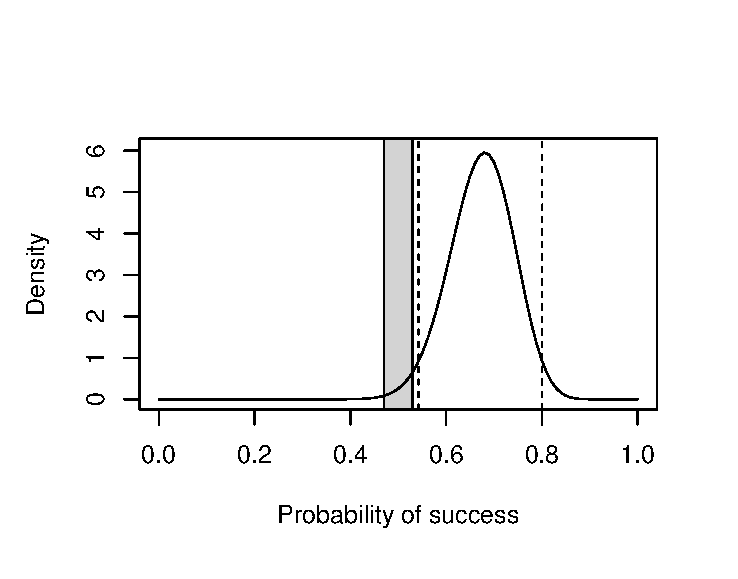
\includegraphics[trim=0 15 30 40,clip,scale=.7]{p/probs.eps}\\
    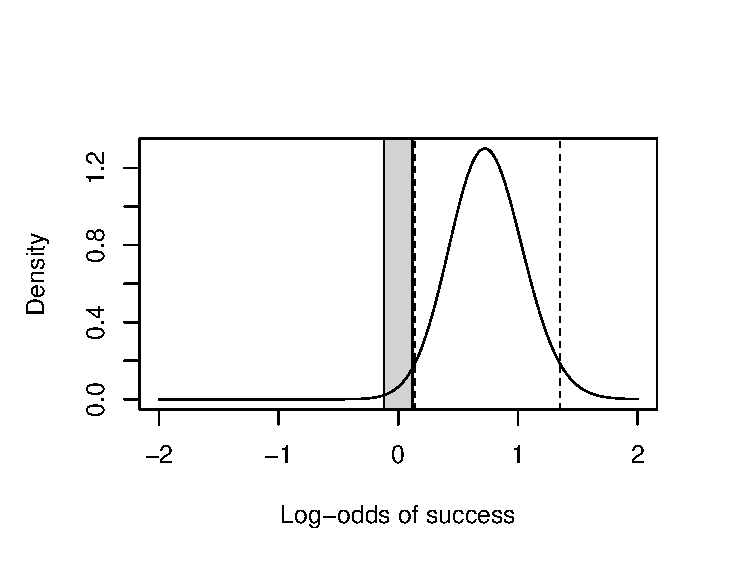
\includegraphics[trim=0 15 30 40,clip,scale=.7]{p/log_odds.eps}\\
    \includegraphics[trim=0 15 30 40,clip,scale=.7]{p/odds.eps}
    \caption{An illustration of the \hdr{}. The shaded region indicates the ROPE, and the dashed line indicates the HDI of the respective posterior distributions. \textbf{Top.} $\theta$ parameterization. Test value is .50, with ROPE from .47 to .53. The 95\% HDI does not intersect the ROPE, leading to rejection of the null hypothesis. \textbf{Middle.} $\logit(\theta)$ parameterization. Test value is $\logit(.50)=0$, with ROPE from $\logit(.47)\approx-.12$ to $\logit(.53)\approx.12$. The 95\% HDI does not intersect the ROPE, leading to rejection of the null hypothesis. \textbf{Bottom.} $\oddss(\theta)$ parameterization. Test value is $\oddss(.50)=1$, with ROPE from $\oddss(.47)=.887$ to $\oddss(.53)=1.128$. The 95\% HDI intersects the ROPE, leading to withholding judgment.}
    \label{fig:ropes}
\end{figure}



    \subsection*{Formal description of the \hdr{}}

We described the \hdr{} informally above, as an assessment of how two intervals overlap. In order to describe the \hdr{}'s problem of incoherence in a precise way we will use the language of statistical decision theory. 
We will begin this section with a brief introduction to decision-theoretic ideas and then discuss how these ideas apply to the \hdr{}.
 
Using the language of statistical decision theory, a hypothesis testing procedure is a type of decision rule in which the decision is a choice between one of the candidate hypotheses. If we use $\delta_T$ to represent the \textit{decision} made for test $T$, then the value of $\delta_T$ corresponds to the hypothesis chosen. For example, in the classic Neyman-Pearson testing framework one sets up a test to choose between the null hypothesis $H_0$ and the alternative hypothesis $H_1$. A test statistic ($X$), acceptance region ($R_0$) and rejection region ($R_1$) are defined. If the test statistic falls in the predefined rejection region, then $\delta_{NP}=1$ and we choose $H_1$; if the test statistic falls in the acceptance region, then $\delta_{NP}=0$ and correspondingly we choose $H_0$.

The \hdr{} is fundamentally a hypothesis testing decision procedure and thus it can also be represented as a decision process. With the \hdr{} we have the same hypotheses as usual: $H_0$ states that the the parameter is (practically) equal to a postulated null value $\theta_0$; $H_1$ states that the parameter takes some value other than $\theta_0$. To test these hypotheses using \hdr{} we define the ROPE, then carry out estimation of the parameter and examine if its posterior density function shows considerable overlap with the ROPE. If the areas of high density mainly lie within the ROPE, $H_0$ is accepted. If the areas of high density are largely outside the ROPE, $H_1$ is accepted. The intuition behind this procedure is seemingly straightforward: If the most plausible parameter values are practically equivalent to the null value, then it makes sense to accept it for practical purposes. Likewise, if the most plausible parameter values are not practically equivalent to the null, then reject it.

The overlap of the ROPE and the posterior distribution is formally determined by constructing a 95\% highest density interval (HDI) for the test parameter. An HDI is a set consisting of 95\% of the posterior mass, with the specific property that every parameter value in the interval has higher posterior density than any value outside the set. Formally, an HDI consisting of $100\alpha\%$ of the posterior mass is defined as the set  
\begin{equation}
    HDI^\alpha = \{\theta:p(\theta|D)>k_\alpha\}\label{eq:hdi}
\end{equation}
for some $k_\alpha$ chosen to satisfy the constraint $P(HDI^\alpha)=\alpha$ \cite{druilhet2007}. For notational convenience, if the $\alpha$ being used is the standard .95 we will simply write ``$HDI$'' without the superscript. 

Formally, we define the decision rule associated with the \hdr{} as follows:
\begin{equation*}
    \delta =
    \begin{cases}
    1 & \text{if HDI} \cap \text{ROPE} = \emptyset \\ %That is an ugly negation slash but I can't find a better looking one atm
    -1 & \text{if HDI} \subset \text{ROPE}\\
    0 & \text{otherwise}.
    \end{cases}
\end{equation*}
In the \hdr{} decision rule, $\delta=1$ corresponds to rejection of $H_0:\theta=\theta_0$ and $\delta=-1$ refers to its acceptance. $\delta=0$ refers to the case there is partial overlap of the sets and one must withhold judgment about the status of the null hypothesis and (if possible) collect more data until one of the other conditions is met.

Let us now revisit the hamster example using this new language. In presenting their results, Avery showed that the HDI and ROPE did not intersect for testing $\theta=.50$, and thus made the decision $\delta=1$ and rejected the null hypothesis. Blair came to a similar conclusion for testing $\logit(\theta)=0$, but the evidence did not appear as conclusive. Cassidy concluded that the HDI and ROPE partially overlapped for testing $\oddss(\theta)=1$, respectively, and thus made the decision $\delta=0$ and withheld judgment. Thus, despite having the same information, the triplets come to different conclusions about logically equivalent hypotheses despite having all of the same information. In the next section, we will provide some critical background on probability theory and use it to explain why the \hdr{} leads to such instances of incoherence. 

\section*{Why is the \hdr{} incoherent?}

We will now explain the cause of the incoherent behavior exhibited by the \hdr{}. A central idea is that the procedure requires the user to find a set of parameters with ``high'' posterior density, but that there is no unique set of parameter values with the highest density. Density is a property that is determined by the parameterization of the model, which is an explicit choice made by the user of the test. As we have seen in our examples above, different choices of parameterization lead to different regions of the model with high density, which in turn leads to different conclusions from the procedure.

To understand why this happens, we will first review the fundamental relationship between probability and probability density. Then, we will show the difference in the way probability and probability density behave when converting from one parameterization to another. Finally, we will return to the \hdr{} and show how it is affected by these considerations.  
    
   \subsection*{Density and probability}


\begin{figure*}[t]
    \centering
    \includegraphics[width=.85\textwidth]{idunno.pdf}
    \caption{An illustration of how transformation affects the CDF and PDF. \textbf{Top left.} The CDF of a normally distributed $\theta$. \textbf{Top right.} The CDF resulting from applying the transformation $\exp(\theta)$. \textbf{Bottom left.} The PDF of a normally distributed $\theta$. \textbf{Bottom right.} The PDF resulting from applying the transformation $\exp(\theta)$.}
    \label{fig:normals}
\end{figure*}

As an illustrative example, imagine that we are testing whether the mean of a normal distribution is equal to zero or not. The posterior distribution we obtain for $\theta$ from our analysis happens to be the standard normal distribution. The cumulative distribution function for a standard normal is shown in the top left panel of Figure~\ref{fig:normals}. This function tells us for any given candidate $\theta$, the posterior probability that the ``true'' $\theta^*$ is less than $\theta$. For example, for $\theta=0$, we have $P(\theta^*<\theta|D) = .50$. This is seen in the graph by the height of the cdf curve for $\theta=0$ being at .50. We will use $F(\theta|D)$ as notation for the cdf.

Recall that probability theory is fundamentally a collection of rules for assigning numbers between 0 and 1 to various sets. The cdf tells us how much probability is associated with the set of parameters whose values fall below a candidate $\theta$. Using this function, we can find the probability of other sets; the probability that $\theta$ is between any two limits $\theta_1$ and $\theta_2$ ($\theta_1<\theta_2$) can be obtained by finding how much the cdf increases as we move from $\theta_1$ to $\theta_2$; we subtract $F(\theta_1|D)$ from $F(\theta_2|D)$ to get $P(\theta_1<\theta^*<\theta_2|D)$. For instance, we take $\theta_2=.6$ and $\theta_1=.4$, then $F(.6|D)=.73$ and $F(.4|D)=.66$, giving $P(.4<\theta^*<.6|D)=.07$. 

When the parameter space is continuous, the probability of any individual point is zero. We can then look at the probability density, which tells us how much probability is concentrated ``near'' a given parameter value. The idea of probability density is directly analogous to physical concepts of density, in that it tells us how much (probability) mass exists in a given region of some space. Consider our example with the standard normal posterior for $\theta$. We could take a small window $\Delta \theta$ around each $\theta$ that spans .1 below and .1 above, and find the probability that $\theta^*$ is between those limits. Some examples are drawn on the top left panel of Figure~\ref{fig:normals}.
Regions that have more probability around them have greater density.

``Near'' $\theta=-1$, there is $5\%$ of our total probability. ``Near'' $\theta=0$ there is $8\%$ of our total probability. This distribution is symmetric around 0, so ``near'' $\theta=1$, there is again $5\%$ of our total probability. If we take these amounts and divide them by the length of the window $\Delta \theta$, we have an idea of how densely the probability is packed around each of these values. We can compute the density of these windows around  $-1$, 0, and $1$ to be .25, .4, and .25, respectively. 

Thinking in terms of the cdf, how dense a region is around a parameter corresponds to how steeply the function rises near that point. The idea of probability density follows this line of thinking into the limit of smaller and smaller windows around $\theta$ values; we look at how much the cdf's value is changing with an infinitesimally small change around the parameter value. In other words, we can look at the slope of the cdf at a given parameter value to find its density. Thus, the posterior density function is the derivative (slope, or rate of change) of the cumulative density function. In this way, an individual parameter value can have a non-zero density, which critically distinguishes probability density from probability.

To summarize, the density of candidate parameter values is determined by first defining a window length to be applied to the regions of $\theta$ (i.e., $\Delta\theta$), finding the probability mass within that window, and then passing on to a limit. This results in taking the derivative of the cdf, telling us how much probability exists in a very small window ``near'' each candidate $\theta$ value. As we can see for our standard normal example, the highest-density point (i.e., the mode) is at $\theta=0$ and the density gradually and symmetrically decreases in either direction.

The difference in the way transformations act on probabilities and probability densities is central to our argument. Equivalent sets of parameters must naturally have equivalent probabilities, but their densities can be quite different.

    
   \subsection*{Reparameterization and transformation of variables}
Probability density quantifies how much probability mass is ``near'' a point in the support of a probability distribution. When the probability distribution is a prior or posterior distribution of a parameter, it is tempting to think of the density as a measure of how ``plausible'' each parameter value is. However, this line of thinking fails when we realize that a parameterization of a model is merely an indexing system of a family of distributions that could have generated the data. Usually when we talk about inference, we make reference to parameter values such as $\theta$, but what is being tested is the data generating process for the data, $f(x|\theta)$. For example, in a $t$-test we may make an inference on whether the difference between group means $\mu_1$ and $\mu_2$ equals zero, but this is merely an expedient way of determining whether $f(x|\mu_1)$ is the same function as $f(x|\mu_2)$. Parameters do not exist outside of a model for some data generating process. 

When we think of parameterizations as indices of data generating processes, it becomes clear that we have to make a choice of which index to use in any given case. It may be that we choose based on convention or ease of interpretability, but we must make a choice; there is no God-given parameterization. And in making our choice, we must recognize that other analysts may make different choices. That is, we may prefer to think of the model in terms of a $\theta$, but someone else may prefer to think in terms of $\psi$ that is some function of $\theta$. In the case that this function is bijective (both one-to-one and onto), we can say that $\psi$ is a \textit{reparameterization} of the model based on $\theta$. 

Let us now consider what happens to our standard normal posterior distribution when we reparameterize the model in terms of $\exp{(\theta)}$. 
The top right panel shows the cdf of the posterior distribution for this new parameterization. Note that the only change is to scrunch and stretch the axis in different regions. 
The height of the curve has no need of adjustment. Naturally, the probability that $\theta<0$ is just the probability that $\exp{(\theta)}<1$. This makes sense, as all we have done is assigned a new labeling scheme for the model, going from $f(x|\theta)$ to $f(x|\psi)$.
For example, the data generating processes that have a $\theta$ smaller than 0 are precisely those that have a $\psi$ less than 1. 
 
In contrast to the simple way probability is maintained through transformation, the new density is not as straightforward.
Recall that density is telling us how much probability is ``near'' different parameter candidates, and what is considered ``near'' a parameter value is defined as a window of width $\Delta$.
The critical problem for thinking about plausibility in terms of density is this: \textit{data generating processes that are ``near'' one another in terms of $\theta$ may not be nearby in terms of $\psi$}. 

Consider three the $\theta$ values of $-1$, $0$, and $1$. In this space (represented by the axis in Fig.~\ref{fig:normals}), the data generating process corresponding to $\theta=-1$ and $\theta=1$ are equally far from the one corresponding to $\theta=0$.
But the data generating process corresponding to $\psi=\exp{(0)}=1$ is now much closer to the one corresponding to $\psi=\exp{(-1)} = .37$ than it is to $\psi=\exp{(1)}= 2.7$.
However, critically, the probability mass of this interval must stay the same, as equivalent sets must have equal probabilities. Thus, the probability mass in the smaller region of $\psi$ between $\exp{(-1)}$ and $\exp{(0)}$ must be more dense than the equally probable but more spread out region between $\exp{(0)}$ and $\exp{(1)}$. This is the central idea of density: the same amount of mass in a smaller region is more dense. 

The story is the same as we shrink the window $\Delta\psi$ in the limit to find the density function. Because the probability mass has been stretched and scrunched differently in different regions of parameter space, some data generating processes that had high (low) density when expressed in terms of $\theta$ may have low (high) density when expressed in terms of $\psi$.
From the $\psi$ perspective, the densest region of parameter space is at $\exp{(-1)}$. The data generating process corresponding to $\psi=\exp{(-1)}$ has the most probability ``around'' it. 

So far we have given an intuition of the idea of how posterior density changes when we transform our parameterization or representation of the model. Essentially, we have to ensure that we account for the stretching being done to the parameter space; regions that stretch out must become less dense, and regions scrunching up must become more dense. 
In the limit, as we look at smaller neighborhoods around the parameter values, we have to make finer grained adjustments to the density. The limiting adjustment is a factor called a \textit{Jacobian} that corrects the density up or down to the extent that the neighborhood around the given parameter is shrinking or expanding (see the subsection ``The Jacobian and coherence''). 

The Jacobian can have a very different effect on different regions of the new parameter space depending on the transformation. It is perhaps instructive to see how the Jacobian works for a few points in the transformation of the parameter spaces for Avery and Cassidy from our hamster example earlier. In transforming from $\theta$ to $\oddss(\theta)$, calling $\gamma={\theta}(1-\theta)^{-1}$, the Jacobian is $(1+\gamma)^{-2}$. The point $\theta=.50$ for Avery goes to the new point $\gamma=1$ for Cassidy, and in doing so it undergoes a density adjustment factor of $(1+1)^{-2} = 1/4$. The point $\theta=.70$ for Avery goes to the point $\gamma=7/3$ for Cassidy, with a Jacobian adjustment of $(1+7/3)^{-2}=.09$. Finally, the point $\theta=.90$ goes to the new point $\gamma=9$ with a Jacobian adjustment of $1/100$.  
The Jacobian is acting more strongly on the larger values of the parameter because the transformation of the space becomes more exaggerated as we approach the boundary of $\theta$. Consider that $\theta=.9$ goes to $\gamma=9$, $\theta=.95$ goes to $\gamma=19$, and $\theta=.99$ goes to $\gamma=99$. The probability around these points is being stretched across larger and larger regions of odds, so the density must be adjusted downwards accordingly. This differential adjustment due to the Jacobian will generally lead to a different set of parameter values having the highest density.

If we were to think of plausibility in terms of density, we would have to interpret the transformation from one parameterization to another as providing some new information. It would be as if the Jacobian is another source of data. But, critically, the adjustment due to the Jacobian does not introduce any new information; its sole purpose is to ensure that the probability density function integrates to~1. 

\subsection{The Jacobian and coherence} \label{subsection:jacobian}
We now give a formal definition of the Jacobian in the context of the log-normal example above. If a univariate random variable $X$ has probability density function $f_X(x)$, then the density function of the random variable $Y=g(X)$, for a smooth function $g$ with inverse $X = h(Y)$, is 
\begin{equation}\label{eq:jacobian}
f_Y(y) = f_X(h(y))  \left|J(y)\right|.
\end{equation}
The factor $J(y) = dh(y)/dy$ is the Jacobian of the transformation, and rescales the density function to ensure that the total probability mass remains~1. The Jacobian factor is a function of the new parameter, meaning that its value depends on where in the parameter space we are; neighborhoods that are shrinking will have a Jacobian greater than~1, and neighborhoods that are expanding will have a Jacobian less than~1.

Let us continue with our example of transforming from a normal random variable to a log-normal. Let $X$ follow a normal distribution with mean $\mu$ and variance $\sigma^2$, i.e., $X\sim N(\mu,\sigma^2)$. The density function of $X$ is 
\begin{eqnarray*}
f_X(x) = \frac{1}{\sqrt{2\pi\sigma^2}}\exp\left\{-\frac{1}{2\sigma^2}(x-\mu)^2\right\},
\end{eqnarray*}
for $-\infty < x < \infty$. If we were to consider where the mode of this distribution is, we would find the value of $x$ making $\exp\{-(x-\mu)^2\}$ the largest, which can be shown to be when $x=\mu$.  

Table~\ref{tab:transformations} shows the Jacobian for many common transformations. The change of variable $Y=e^X$ corresponds to the fourth row of the table with $a=1$. Thus, we have inverse $X=\log(Y)$ and a Jacobian equal to $1/Y$. Equation~\ref{eq:jacobian} tells us that the density function of $Y$ is given by
\begin{eqnarray*}
f_Y(y) &=&  \frac{1}{\sqrt{2\pi\sigma^2}}\exp\left\{-\frac{1}{2\sigma^2}\Big(\left(\ora{\log(y)}\right)-\mu\Big)^2\right\}\cdot\left|\blu{\frac{1}{y}}\right|\\
&=& \frac{1}{\blu{y}\sqrt{2\pi\sigma^2}}\exp\left\{-\frac{1}{2\sigma^2}\Big(\ora{\log(y)}-\mu\Big)^2\right\},
\end{eqnarray*}
for $0<y<\infty$. It can be shown that the mode of this new density is at $y=\exp{(\mu-\sigma^2)}$. 

If we were to interpret density as an indication of ``plausibility,'' then the point with highest density should be considered the ``most plausible'' value of a random variable (i.e., the mode). We would then have to simultaneously believe that the most plausible value of $X$ is $\mu$, but that the most plausible value of $Y=\exp{(X)}$ is not $\exp{(\mu)}$, but the potentially very different $\exp{(\mu-\sigma^2)}$. These two beliefs are contradictory, so treating density as a measure of plausibility leads to logical absurdity and is not a coherent system of reasoning.


\begin{table}[tb]
\centering 
\caption{Some common transformations and their corresponding Jacobian factors. The first column lists various transformations in the form $Y=g(X)$. The second column lists the inverse functions, $X=h(Y)$. The third column lists the Jacobian factors corresponding to each transformation, obtained by taking the derivative of the corresponding inverse function (see the explanation in the main text). Note that $\Phi$ is the normal CDF and $\phi$ is the normal PDF. Finally, the rightmost column indicates whether the transformation is linear or nonlinear -- the scale dependence of the \hdr{} occurs only with nonlinear transformations.}
\label{tab:transformations}
\begin{tabular}{llll}\hline
Transformation & Inverse function & Jacobian & Linear  \\ \hline
$Y = g(X)$ & $X = h(Y)$ & $J(Y) =\frac{dh(Y)}{dY}$ &  \\\hline
$Y=aX +b$  & $X= \frac{Y-b}{a}$ & $J(Y)=\frac{1}{a}$ & Yes \\
$Y= X^a$   & $X = Y^{1/a}$      & $J(Y)=\frac{1}{a} Y^{\frac{1-a}{a}}$ & No \\
$Y= X^{1/a}$ & $X = Y^{a}$ & $J(Y)=a Y^{a-1}$ & No \\
$Y = e^{aX}$ & $X = \frac{1}{a}\log(Y)$ & $J(Y)=\frac{1}{aY}$& No \\
$Y = a\log(X)$  & $X = e^{Y/a}$ & $J(Y)=\frac{1}{a}e^{Y/a}$& No \\
$Y = \frac{X}{1-X}$ & $X = \frac{Y}{1+Y}$  & $J(Y)=\frac{1}{(1+Y)^2}$ & No\\
$Y = \frac{X}{1+X}$ & $X = \frac{Y}{1-Y}$ & $J(Y)=\frac{1}{(1-Y)^2}$& No\\
$Y = \log\left(\frac{X}{1-X}\right)$ & $X = \frac{1}{1+e^{-Y}}$ & $J(Y)=\frac{e^{-Y}}{\left(1+e^{-Y}\right)^2}$& No \\
$Y = \frac{1}{1+e^{-X}}$ & $X = \log\left(\frac{Y}{1-Y}\right)$ & $J(Y)=\frac{1}{Y(1-Y)}$& No\\
$Y = \Phi^{-1}(aX+b)$ & $X = \frac{\Phi(Y)-b}{a}$  & $J(Y)=\frac{1}{a}\phi(Y)$& No\\[.5ex]\hline
\end{tabular}
\end{table}

\subsection*{Issues with the density-based \hdr{}}

As we have shown in the discussions above on density and transformation, regions of parameter space having ``high'' or ``low'' density depends on how we choose to parameterize the data generating process. The relative ordering of density can change drastically across reparameterizations of the model, meaning any inferences based directly on density are essentially artifacts of a statistically arbitrary parameterization choice. 

The \hdr{} relies on the determination of overlap between a high-density region and an ``equivalency'' region of the parameter space. The issue with the procedure is now apparent: regions of parameter space can have high density in one parameterization and low density in another, meaning the location of the HDI relative to the ROPE is dependent on an arbitrary parameterization choice.  Thus, the inference one draws from the \hdr{} is not invariant to reparameterization of the model. 

In fact, the non-invariance of the \hdr{} to reparameterization suggests that the way we have written the decision rule associated with the procedure in the earlier section is incomplete; the entire decision process should be indexed by the parameterization choice made. Thus, the HDI should be explicitly $\text{HDI}_\theta$, the ROPE should explicitly be $\text{ROPE}_\theta$, and the decision rule should be explicitly $\delta_\theta$. Thus, in terms of decision theory, the problem with the \hdr{} is that with the same data and prior, it is not the case that the decision $\delta_\theta$ will necessarily be equal to the decision $\delta_\psi$ associated with a reparameterization of the model. Different analysts with the same information can come to different conclusions based solely on their choice of parameterization.

\subsection{Computational demonstration of transformation incoherence}

To help develop a deeper understanding of these technical points, we will now demonstrate how the transformation incoherence of the \hdr{} can be seen in practice using modern computational tools. 
Modern Bayesian analysis is done using computational tools such as MCMC \cite{vanravenzwaaijSI}. These computational methods are able to generate samples from a posterior distribution, which can then be used to draw inferences from the data. We can obtain the posterior samples from a reparameterized version of a model by applying the transformation directly to the original posterior samples (treating them as derived parameters). For example, if we can obtain samples from the posterior distribution of a binomial rate $\theta$, and we wish to draw inferences about some transformation $g(\theta)$, we can simply apply the transformation to each sample from the original posterior to obtain the posterior samples for the derived $g(\theta)$. 

Suppose we have 1000 posterior samples for $\theta$, denoted $\theta_k$ for $k=1,2,\dots,1000$, ordered from smallest to largest. The 95\% highest-density interval for $\theta$ can be found in two steps. Start by taking the first sample and the 950th sample and check the length of the interval they form, $\theta_{950} - \theta_1$. Then, check $\theta_{951}-\theta_2$, $\theta_{952}-\theta_3$, and so on in sequence until the length of all such possible intervals are computed. The shortest such interval will be the highest density interval. 

Consider the reparameterization $\logit(\theta)=\log\left(\frac{\theta}{1-\theta}\right)$. To obtain posterior samples from $\text{logit}(\theta)$, we simply apply the transformation to each $\theta_k$. The reparameterization will not change the rank order of the samples, it will simply put them into a new scale. The effect of this transformation is shown in Figure~\ref{fig:transformation}. Here we are implementing the \hdr{} to test $\theta=.5$ with a shaded ROPE of $(.40, .60)$. The top panel shows the posterior distribution of 1000 samples taken from a beta$(10,2)$ distribution. The bottom panel shows the posterior distribution of the posterior samples after applying the $\logit$ transformation. The lines connecting the two panels show how values of $\theta$ are mapped into the space of $\logit(\theta)$. Notice that equally spaced values of $\theta$ do not remain equally spaced after the reparameterization: values near $\logit(\theta)=0$ are closer to each other than points at the extremes. The effect of the reparameterization on the ROPE is shown by the shaded region connecting the panels. 

When we obtain the HDI for the reparameterization, the procedure operates the same way on the transformed samples. But, critically, the relative distances between the transformed samples will not be preserved due to the fact that samples near the middle of the scale are now closer to each other than samples near the extremes. This means that some intervals that were relatively longer in the original parameterization may be shorter in the new one, and vice versa. The effect of this transformation is shown by the dashed lines connecting the two panels of Figure~\ref{fig:transformation}. Notice the shearing effect when compared to the rest of the traced lines. This shearing force is the Jacobian in action. 

Because the HDIs must account for the density adjustment due to the Jacobian, they transform at a different angle. The transformation incoherence of the \hdr{} is demonstrated where the lower bound of the HDI crosses into the ROPE area. 

The thick solid lines connecting the two panels show the 2.5\% and 97.5\% quantiles of the posterior distributions, which together form a central 95\% quantile interval. As we explain later on in ``Easy-to-implement modifications of the \hdr{} test to achieve coherence'', quantiles are based on probabilities and therefore inherit coherence. The transformation coherence of quantile intervals can be seen by them operating at the same angle of the rest of the transformation. The quantile interval lines cross with the sheared HDI lines because the quantile intervals are unaffected by the Jacobian factor.

\citeA{Kruschke2010Book} provides code to produce HDIs from MCMC output and produce figures summarizing the results. In the appendix we provide code to replace the HDIs with quantile-based intervals. This simple fix brings the procedure back to a state of coherence while allowing the user to continue using the computational framework provided by \cite{Kruschke2010Book} with minimal interruption.

\begin{figure}
    \includegraphics[angle=-90]{p/transformation.eps}
    \caption{\textbf{Top.} Posterior distribution over the probability of success $\theta$. \textbf{Bottom.} Posterior distribution over the transformation logit($\theta$). The connected points highlight the uneven shrinking of the logit transformation, as does the gray polygon marking the ROPE limits in both scales. The solid black lines correspond to the quantile interval, which retains the original overlapping with the ROPE as the relative order of the posterior samples remains the same since the logit transformation is monotonic. In contrast, the HDI, indicated by the dashed lines, switches from non-overlapping in the original scale to overlapping after the logit transformation.}
    \label{fig:transformation}
\end{figure}

\section*{Additional examples}

Recognizing that it is possible to expose the scale sensitivity of the HDI by deriving the Jacobian of the transformation, we can now easily show other examples of models used in psychological science that are susceptible to incoherence if \hdr{} is used.  In this section, we provide  additional examples of statistical models whose varying parameterizations lead to incoherence.

\subsection*{Three parameterizations of the Rasch model}

The Rasch model \cite{Rasch1960} is one of the most common models in item response theory, with many useful applications and theoretical results well known to psychometricians.  Its most typical parameterization is the one shown first in the equations below, where the probability of person $p$ answering correctly on item $i$ is a logistic function of the difference between $p$'s ability $\theta_p$ and $i$'s difficulty $\beta_i$: $P(X = 1) = \left[1+e^{-(\theta_p-\beta_i)}\right]^{-1}$. However, at least two other parameterizations exist and have their own specific use cases (see, e.g., \citeNP{Batchelder1998,CrowtherEtAl1995}): $P(X = 1) = {\alpha_p}\left(\alpha_p + \delta_i\right)^{-1}$ and $P(X = 1) = {a_p b_i}\left[a_pb_i+(1-a_p)(1-b_i)\right]^{-1}$.

Here, $\delta_i = e^{\beta_p}$, $\alpha_p = e^{\theta_p}$, $a_p      = \left[1+e^{-\theta_p}\right]^{-1}$, and $b_i = \left[1+e^{-\beta_i}\right]^{-1}$.
The Jacobians associated with these transformations are shown in Table~\ref{tab:transformations}.  Since the associated Jacobians are a function of the parameters themselves, these transformations distort the scale in a way that causes incoherence when using the \hdr{}.

\subsection*{Kimura phylogenetic model}

Moving outside of research psychology, this example concerns DNA evolution.  Models of DNA evolution could be thought of as descriptions of the process of nucleotide substitution \cite{Zwickl2004}. One model family of DNA evolution known as the ``Kimura family model'' assumes that  all four nucleotides will be equally common, that the eight types of transversions will occur at one rate, and that the four types of transitions will occur at a second rate. Within the confines of these assumptions, the Kimura model family can generate predictions ranging from all substitutions being transversions to all being transitions.
%
A key parameter in this model family is the transition transversion rate ratio $\kappa$, which is used to describe this range of possibilities. The two ends of the spectrum of predicted
substitution patterns are specified by a $\kappa = 0$ (all transversions) and $\kappa = +\infty$ (all transitions).
%
An alternative parameterization of this model family characterizes instead the proportion $\phi$ of substitutions that are transitions. This parameter can be written as a function of $\kappa$:
$\phi = \kappa (2 + \kappa)^{-1}$. 
The Jacobian corresponding to this reparameterization is $J(\phi) = 2(1 - \phi)^{-2}$, which is clearly nonlinear.

\subsection*{The circular drift-diffusion model}

The circular drift-diffusion model \citep[CDDM;][]{smith2016diffusion} is a process model used to describe response and response time data collected in tasks where the decision space is a circle. The model belongs to the category of sequential sampling models that assume that individuals accumulate information about the stimuli presented from the moment the trial starts until they are ready to input a response. 

There are two parameterizations of the model that are considered equivalent, one describing the drift vector in terms of drift angle $\driftangle$ and drift length $\driftlength$, and the other describing it in terms of horizontal drift $\mux$ and vertical drift $\muy$. Moving between these two parameterizations involves transforming between Cartesian and polar coordinates:
$\mux = \driftlength \cos\left(\driftangle\right)$ and 
$\muy = \driftlength \sin\left(\driftangle\right)$.

The case of reparameterization with multiple interdependent parameters is slightly more complicated than our previous examples. The scaling factor that we need is the absolute value of the determinant of the transformation, which is:
\begin{eqnarray*}
||J|| &=& \begin{vmatrix} \begin{vmatrix}
   \frac{\partial \mux}{\partial \driftlength}&\frac{\partial \mux}{\partial \driftangle}\\
   \frac{\partial \muy}{\partial \driftlength}&\frac{\partial \muy}{\partial \driftangle}
    \end{vmatrix} \end{vmatrix}\\ &=& \begin{vmatrix} \begin{vmatrix}
   \frac{\partial \driftlength \cos \driftangle}{\partial \driftlength}&\frac{\partial \driftlength \cos \driftangle}{\partial \driftangle}\\
   \frac{\partial \driftlength \sin \driftangle}{\partial \driftlength}&\frac{\partial \driftlength \sin \driftangle}{\partial \driftangle}
    \end{vmatrix} \end{vmatrix}\\ &=&
    \left|\left(\cos \driftangle \cdot \driftlength \cos \driftangle \right)-\left(- \driftlength \sin \driftangle \cdot \sin \driftangle \right)\right|=\driftlength.
\end{eqnarray*}
Again the transformation is nonlinear and the Jacobian is a function of a parameter.

However, the multidimensionality of the CDDM leads to additional complications.  We could continue and derive the multidimensional posterior distribution corresponding to the new parameterization, but how to conduct the \hdr{} at that point is less immediate.  We suspect most researchers would prefer to perform the \hdr{} using the marginal posterior of the parameter of interest. This involves integrating out any other non-focal parameters, such as $\driftlength$. This adds more layers of complexity to the transformations involved, and we do not discuss them further here. Suffice it to say that the multiparameter \hdr{} is fraught with nonlinear relationships. 

The three examples above serve to illustrate the ubiquity of nonlinear reparameterizations possible for scientific models across psychology and related fields. Despite the apparently common preference to represent models using certain ``canonical'' parameterizations, ultimately \textit{the epistemic content of a model is not in its parameters but in the distributions it generates over data}. There is always an alternative parameterization that could be meaningfully understood; good methods should give us the same conclusions across them all.

Broadening our scope from these example models, we conclude by pointing out that the ubiquitous framework of generalized linear modeling relies on the frequent application of ``link functions'' that map parameters between scales -- often from one scale that is natural for the parameter (e.g., a probability that lives between $0$ and $1$) to one that is convenient for regression (e.g., its logit transform that lives on the full real line).  All nontrivial link functions are nonlinear, and hence the \hdr{} will be incoherent in those common cases.

\section*{Easy-to-implement modifications of the \hdr{} for achieve great coherence}

The incoherence of the \hdr{} lies entirely in the choice of the HDI as a reference to compare with the ROPE. Because the HDI is defined with regard to the specific parameterization of the posterior distribution, and because density of any given data generating process can be high or low depending on parameterization, the set that we end up comparing to the ROPE depends on a statistically arbitrary choice. This means that any conclusions we draw from our hypothesis testing procedure depends critically on a choice of how the model is described. 

The transformation incoherence we have highlighted here can only occur when sufficient posterior mass lies inside or outside of the ROPE. By definition, a 95\% HDI is a set of parameter values with probability .95. This probability will remain inside/outside the ROPE no matter how we choose to reparameterize. Thus, we cannot have a case where the conclusion from an \hdr{} flips from rejection to acceptance -- the maximum extent of the incoherence is to change a rejection or acceptance into an inconclusive result (or vice versa). This is still not very comforting, because any opportunity for inferences to change arbitrarily based on statistically irrelevant choices indicates a fundamental weakness of a procedure. In the remainder of this paper we will suggest some changes that could be made to the \hdr{} test to achieve coherence.

The \hdr{} suffers from transformation incoherence precisely because it uses density-based interval estimates. As we have demonstrated, the regions of parameter space with high density in one parameterization can have low density in another. This weakness can be overcome with a simple modification of the procedure: transitioning to probability-based decision rules. Because probability theory itself is coherent, methods derived directly from it will inherit that coherence. 

\subsection*{Quantile intervals}

The simplest transition to probability-based inference is to use quantile intervals, which already happen to be a very common output in Bayesian software.  These intervals are constructed by taking the inner $100\alpha\%$ of the probability mass of the posterior distribution, leaving $\left(\frac{1-\alpha}{2}\right)\%$ of the mass outside the interval on either end. 

Quantile-based intervals will naturally be transformationally coherent, because they are based directly on probability. Using the cdf, a quantile interval can be constructed by finding the parameter values with heights equal to .025 and .975. As we have seen, the only change that occurs in a cdf during a transformation is to stretch and scrunch the points along the x-asis -- the function values at those points remain unchanged. Thus, tests based on quantile-interval endpoints will be transformationally coherent.

Transitioning to probability-based intervals is an easy fix to the problem of transformation incoherence because they are already in broad use. Most software that performs Bayesian inference, such as JAGS and Stan, will by default produce these intervals in a model summary. These are computationally easy to produce because all one needs to do is note which posterior samples correspond to the appropriate sample quantiles. Almost no software is producing density-based intervals by default, probably because it involves additional computational steps to find the shortest such interval.


\subsection*{Posterior mass in the ROPE}

Once we move to a quantile-based interval for use in the \hdr{} test, an even easier alternative solution presents itself. Why not simply compute the posterior probability that the parameter is in the ROPE? The interval comparison required by the ROPE test is superfluous at this point. Recall that a 95\% quantile interval is constructed by taking 2.5\% and 97.5\% quantiles of the cdf. But most posterior distributions are unimodal, meaning this interval is generally going to be a contiguous set of parameter values. Thus, for the interval to not intersect the ROPE, the probability the parameter is in the ROPE must be at most 2.5\%. Thus, we could simply use a decision rule that rejects the null hypothesis when the probability it is in the ROPE is sufficiently low, and accept it when it is sufficiently high. 

Indeed, directly computing a probability is the natural Bayesian approach to such a problem. If we look back at our example with the triplets and their hamster, the set of parameters in the HDIs changed dramatically across the three parameterizations. However, the probability of the ROPE is approximately .02, sufficiently small to cast doubt on the null hypothesis regardless of one's choice of parameterization.  We will present an example of how this approach would impact the conclusions of a recently published result in the next section.

%A direct probability approach has one potential weakness to it. If a sensible and defensible prior distribution is thoughtfully constructed, it is possible that before collecting any data the probability of the ROPE set is sufficiently high or low, meaning the null hypothesis could be accepted or rejected without any need for new data.\footnote{This may also occur with relatively non-informative priors, which spread the probability out thinly over a large region.} We think there are a few reasonable reactions to this situation. If we are already convinced that the null is (not) a sensible estimate for the parameter, then we could acknowledge that this new experiment is not really necessary to answer this research question. Of course, there is nothing to stop a researcher from running the new study and seeing if this inference holds with the addition of new data. But then again, why waste resources testing again something we may already be quite sure about? 

%However, the researcher may still want to run this experiment despite being pretty sure the parameter is (not) effectively null. In this case, one may be more interested in estimating the size of the effect in question and knowing its value with more precision. In this case, a hypothesis test is not relevant anyway, so the probability of the ROPE is not relevant. 

Alternatively to estimating the size of the parameter of interest, one may still be interested in evaluating the statistical evidence for or against the nullity of the parameter% even if its probability is already low or high
. To this end, one can compute the Bayes factor associated with the hypothesis that the parameter is inside versus outside the ROPE. Such a Bayes factor would compare the posterior odds that the parameter is inside the ROPE to the corresponding prior odds, which is computationally convenient if the posterior is obtained via sampling.\footnote{Note that the odds in question are equal to $P(\text{ROPE})/P(\lnot \text{ROPE})$. If one obtains the posterior by simulation, this would correspond to the proportion of posterior samples inside versus outside the ROPE.} This Bayes factor would tell us the extent to which the data are making us more or less confident that the parameter is inside the ROPE. Critically, this Bayes factor would be based on probabilities and thus would trivially maintain coherence.



 \section*{Real-life example}

\citeA{newton2018} present a cluster randomized trial examination of the efficacy of an intervention program designed to reduce cannabis usage among Australian high school students. A total of 2190 students were randomly assigned to one of four possible intervention conditions (including the control condition), with measures related to cannabis usage, related harms, and knowledge taken at baseline, and 6-9 months, 12, 24, and 36 months after the baseline (i.e., post-intervention measures). 

The data analysis presented by the authors focused mainly on the differences between the control group and all intervention conditions. The primary statistical analysis was conducted using multilevel mixed-effects linear models that incorporated individual and group (i.e. school) level random effects. 

The authors found no statistical differences in cannabis usage and related harms between the control and intervention groups. These results were explained as a byproduct of the lower-than-expected prevalence of these behaviors in the overall sample (i.e., $5\%$ of the total students). The authors then implement the \hdr{} to further examine the evidence provided by the data. This decision was motivated by the fact that Bayesian hypothesis testing techniques are known to quantify the evidence in favor of both the null and the alternative hypothesis. 

The \hdr{} was implemented using a multi-level Bayesian logistic regression model to account for the probability of cannabis usage and related harms at a given moment in time for participants in the control and intervention group. They defined a test value for the odds ratio $\theta=1$ and a ROPE of $[0.9,1.1]$. The authors note that the HDI for the odds ratio overlapped partially with the ROPE and thus concluded that the non-significant results found in the primary analysis were ambiguous and not indicative of a lack of intervention's true effect.

The goal of presenting this real-world example lies in contrasting the \hdr{} results with those achievable through using a direct probability approach. Table~\ref{tab:newton} presents results reported by \citeA{newton2018} against a collection of alternative probability-based measures corresponding to the data collected at each moment in time. 

In table~\ref{tab:newton}, the second column presents the median odds ratio and the range of the $95\% \text{HDI}$ as reported by the authors; the third column lists the probability that the odds ratio value is contained in the ROPE $p(\text{ROPE})$; the fourth column shows the probability that the odds ratio is smaller than 0.9 $p(\text{OR}<0.9)$; and the fifth and far-right column shows the probability that the odds ratio is larger than 1.1 $p(\text{OR}>1.1)$. Summing the fourth and the fifth columns we obtain the probability that the odds ratio falls outside of the ROPE (i.e., being either smaller than 0.9 or larger than 1.1), which by the complement rule of probability theory is the same as $1-p(\text{ROPE})$. Probability-derived measures are coherent by definition. 

As we can see, there is a decline over time in the probability that the odds ratio coincides with the ROPE. More specifically, by 24 months, the probability that the odds ratio is practically equivalent to $1$ is only .061, and at 36 months, the probability is only .04. Critically, we note that despite the wide HDIs found at 24 and 36 months, we are relatively confident that the odds ratios at these times are outside the ROPEs.


\begin{table}
\caption{A selection of results of the logistic regression analysis from Newton et al. (2018).}\label{tab:newton}
\begin{tabular}{ccccc}\hline
    Time & OR[median(95\% HDI)] & p(ROPE) & p(OR$<$0.9) & p(OR$>$1.1)  \\\hline
   6m  & 0.87 (0.74 to 1.02) & .351 & .646 & .003\\
   12m & 0.76 (0.54 to 1.02) & .138 & .851 & .011\\
   24m & 0.58 (0.27 to 1.01) & .061 & .913 & .026\\
   36m & 0.45 (0.12 to 0.99) & .040 & .929 & .031\\\hline
\end{tabular}
\end{table}

This real-world example helps to illustrate the advantages of working with direct probability measures, which preserve the intuitive reasoning of the \hdr{} while also guaranteeing its internal coherence.
 
\section*{Conclusion}
We have highlighted a critical flaw with the \hdr{} method: transformation incoherence. This flaw can lead different researchers with the same priors and data to draw different conclusions because they have arbitrarily chosen different parameterizations of the problem. We have shown that the root cause of this incoherence lies with the choice of using highest density intervals in the test. Because these intervals are constructed with reference to a specific density function from one specific parameterization, the change from one chosen parameterization to another causes the the set of highest density points to change; where the original set may have excluded the ROPE, the new set may intersect with the ROPE. 

We are not the first to point out the problems with thinking of density as a measure of ``plausibility.'' However, most discussion tends to focus on the consequences this thinking has on coherent specification of priors. Perhaps the most famous objection to this line of thinking was made by Fisher \cite{lehmann2011fisher}, who argued against the use of uniform priors to represent ignorance because they will only be uniform in one parameterization of a model \cite<for a thorough demonstration see>{ly2017tutorial}. \citeA{Zwickl2004} provide a clear illustration of the problem with taking uniform priors to represent ignorance in the context of the General Time-Reversible Model, in which it common to reparameterize in terms of either $\kappa$ or $\phi = \kappa/(2+\kappa)$. Uniform priors in either $\kappa$ or $\phi$ lead to highly informative priors on the other scale. 

Similar considerations led \citeA{jeffreys1946} to develop the now famous invariant Jeffreys prior rule. \citeA{druilhet2007} propose a class of prior densities that lead to invariant highest density sets, avoiding transformation incoherence of the HDI. However, their solution imposes specific choices of Jeffreys-type priors that may not be desirable or may not even exist in practice for models with sufficient complexity. This led \citeA{druilhet2012} develop new invariant conjugate families of priors which can be applied when the model is a member of the exponential family. 

In addition to issues in prior specification, issues with using density-based loss functions in estimation and testing have been pointed out by \citeA{bernardo2005}. Bernardo argues against using density-based loss functions in favor of a parameterization invariant ``intrinsic'' loss function based on the structure of the likelihood function. Our argument can be seen as an extension of Bernardo's to the specific case of the \hdr{} test. However, we prefer probability-based intervals over ``intrinsic'' intervals, if for no other reason than that they are computationally and conceptually simpler and thus more likely to be adopted in practice. 

We have focused here on the simplest case where this problem arises, namely, models with a single parameter. The potential for incoherent inferences only increases when considering models and simultaneous hypothesis tests of multiple parameters, as the multivariate Jacobian factor must account for stretching and scrunching across all dimensions of the parameter space. 

Critically, all parameterizations of a model are equally valid -- there is no ``one true parameterization'' for any model -- so the inference from the \hdr{} test critically hinges on what may be an arbitrary choice made by the researcher. We suggest a change to the \hdr{} test to remedy this incoherence: use probabilities instead of densities. A direct probability approach is both conceptually and computationally simpler than one based on densities. Probabilities, by their very construction, must lead to coherent inferences. 

\bibliography{references}\null

\newpage
\onecolumn
\appendix
\section{R code for the quantile interval}

It is easy to change existing R code to make use of quantile intervals instead of HDIs.  The function below can be used in the same way as the \texttt{HDIofMCMC} function provided by \citeA[p.~628-629]{Kruschke2010Book}.

\begin{lstlisting}[style=rstyle, 
%caption={Your R Code}, 
label=lst:r-code]
 QIofMCMC <- function(sampleVec,credMass=0.95){
          # Computes the quantile interval from (1-credMass)/2 to 1-(1-credMass)/2, where credMass is the target percentage of posterior samples to be included in the interval.
          # The typical value credMass=0.95 results in an interval from the 2.5% to the 97.5% quantile.
          alpha <- (1-credMass)/2
          lim <- quantile(sampleVec,probs=c(alpha,1-alpha))
          return(lim)
 }
\end{lstlisting}\null

\end{document}
